%Este trabalho está licenciado sob a Licença Creative Commons Atribuição-CompartilhaIgual 3.0 Não Adaptada. Para ver uma cópia desta licença, visite https://creativecommons.org/licenses/by-sa/3.0/ ou envie uma carta para Creative Commons, PO Box 1866, Mountain View, CA 94042, USA.


\chapter{Curvas e trajetórias}\index{curvas e trajetórias}\index{trajetórias}
  Neste capítulo, estudamos funções vetoriais do tipo $\vec{r}(t)$, ou seja, uma função que associa um parâmetro real a vetores no plano ou espaço. Tais função vetoriais, que dependem de apenas uma variável, são os exemplos mais simples que estudaremos. %Na seção \ref{tr}Definimos o triedro de Frenet-Serret e introduzimos os conceitos de curvatura e torção, bem como aplicações na física-matemática.

\section{Funções vetoriais de uma variável - curvas e trajetórias}
Uma função vetorial de uma variável é uma função da forma $$\vec{r}:D\to \mathbb{R}^3,$$ onde $D\subseteq \mathbb{R}$ é o domínio de definição de $\vec{r}$ e $t$ é um parâmetro - podendo ser interpretado como o tempo ou não. Em coordenadas cartesianas, uma função vetorial assume a seguinte forma:
$$\vec{r}(t)=x(t)\vec{i}+y(t)\vec{j}+z(t)\vec{k}$$
\begin{ex}\label{exfv1} São exemplos de funções vetoriais
\begin{itemize}
\item [a)] $\vec{f}(t)=\sin(t)\vec{i}+\cos(t)\vec{j}$
\item [b)] $\vec{g}(t)=t \vec{i}+\cosh(t)\vec{k}$
\item [c)] $\vec{h}(t)=2\cos(t)\vec{i}+4\sin(t)\vec{j}+t\vec{k},~~ 0\leq t \leq 8\pi$
\end{itemize}
\end{ex}  

Uma curva\index{curva} no espaço pode ser representada pelo conjunto de pontos de uma função vetorial $\vec{r}(t)$ não constante em todo o seu domínio. Um ponto $\vec{r}(t)$ de uma parametrização é dito regular se $\vec{r}\!~'(t)\neq 0$. Uma parametrização é dita regular\index{parametrização regular} em $t$ se $\vec{r}~\!'(t)\neq 0$ em todos os pontos. É possível definir orientação para uma curva regularmente parametrizada\index{orientação de uma curva}, a orientação é dada pelo sentido de crescimento do parâmetro $t$. 

\begin{ex}
A função vetorial $\vec{f}(t)=\cos(t)\vec{i}+\sin(t)\vec{j}$ para $0\leq t \leq 2\pi$ descreve  uma circunferência de raio 1 centrada na origem sobre o plano $xy$ orientada no sentido anti-horário.
\end{ex}

\begin{figure}%{0.35\textwidth}
\begin{center}
    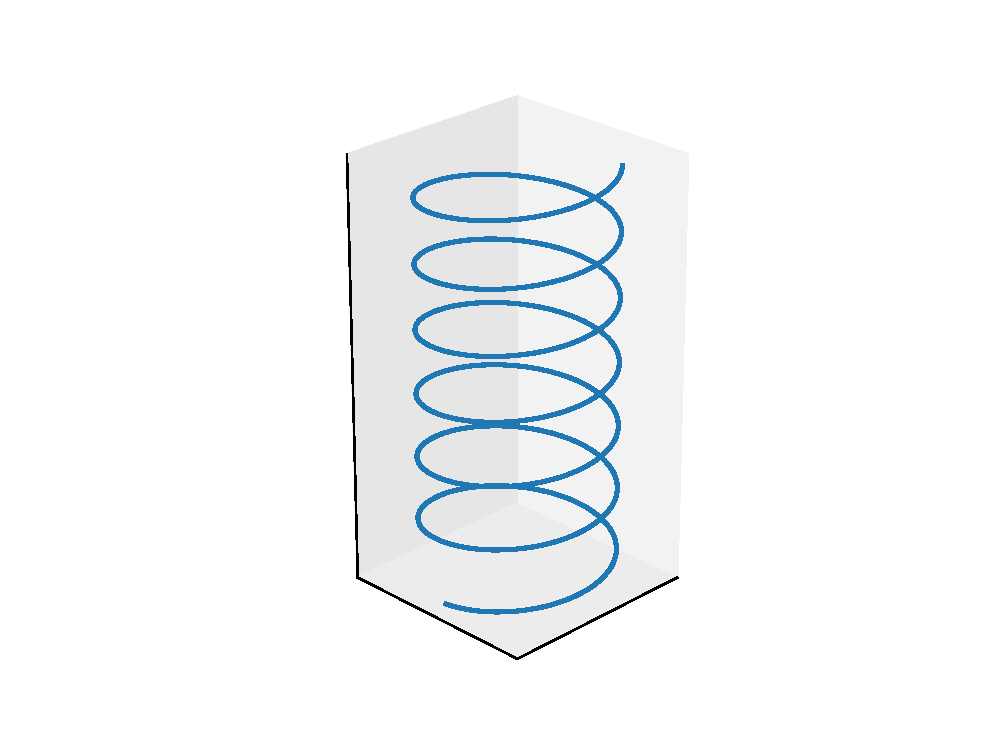
\includegraphics{./cap_curvas/figs/helice}
\caption{\label{helicedex}Hélice circular dextrogira associada à função vetorial do Exemplo~\ref{cap_curvas:exemplo_helice}.}
  \end{center}
\end{figure}

\begin{ex}\label{cap_curvas:exemplo_helice}
A função vetorial $\vec{f}(t)=\cos(t)\vec{i}+\sin(t)\vec{j}+t\vec{k}$ para $ t \in\mathbb{R}$ descreve uma hélice circular, como mostra a figura \ref{helicedex}.
\end{ex}

O limite\index{limite de uma função vetorial de uma variável}, a derivação\index{derivada de uma função vetorial de uma variável} e a integração vetorial\index{integral de uma função vetorial de uma variável} são definidas componente a componente no sistema de coordenadas cartesiano:
\begin{eqnarray}
\lim_{t\to a}\vec{r}(t)&=&\lim_{t\to a}x(t) \vec{i}+\lim_{t\to a}y(t)\vec{j}+\lim_{t\to a}z(t)\vec{k}\label{deflim}\\
\frac{d\vec{r}(t)}{dt}&=&\frac{d x(t)}{dt}\vec{i}+\frac{d y(t)}{dt}\vec{j}+\frac{d z(t)}{dt}\vec{k}\label{defder}\\
\int_{a}^b\vec{r}(t){dt}&=&\int_{a}^bx(t)dt~\!\vec{i}+\int_{a}^by(t)dt~\!\vec{j}+\int_{a}^bz(t)dt~\!\vec{k}\label{defint}\\
\int\vec{r}(t){dt}&=&\int x(t)dt~\!\vec{i}+\int y(t)dt~\!\vec{j}+\int z(t)dt~\!\vec{k}\label{defint2}
\end{eqnarray}

\begin{teo}[Regras de derivação] A derivada de funções vetoriais satisfaz as seguintes identidades:
\begin{enumerate}
\item Se $\vec{r}(t)$ é um vetor constante, então $\vec{r}'(t)=\vec{0}$. 
\item $\frac{d}{dt}\left[\alpha \vec{r}_1(t)+\beta \vec{r}_2(t)\right]=\alpha\frac{d\vec{r}_1(t)}{dt}+\beta\frac{d\vec{r}_2(t)}{dt}$
\item Se $f(t)$ é uma função real, então $\frac{d}{dt}\left[f(t) \vec{r}(t)\right]=f'(t)\vec{r}(t)+f(t)\frac{d\vec{r}(t)}{dt}$
\item $\frac{d}{dt}\left[\vec{r}_1(t)\cdot \vec{r}_2(t)\right]=\vec{r}_1(t)\cdot\frac{d\vec{r}_2(t)}{dt}+\frac{d\vec{r}_1(t)}{dt}\cdot\vec{r}_2(t)$
\item $\frac{d}{dt}\left[\vec{r}_1(t)\times \vec{r}_2(t)\right]=\vec{r}_1(t)\times\frac{d\vec{r}_2(t)}{dt}+\frac{d\vec{r}_1(t)}{dt}\times\vec{r}_2(t)$
\end{enumerate}
\end{teo}
\begin{proof} Os dois primeiros ítens podem ser obtidos diretamente de (\ref{defder}). A verificação fica a cargo do leitor. O item três pode ser obtido de  uma aplicação da regra da cadeia a (\ref{defder})\index{derivada do produto de um escalar por um vetor}:
\begin{eqnarray*}\frac{d}{dt}\left[f(t) \vec{r}(t)\right]&=& \frac{d}{dt}\left[f(t) {x}(t)\vec{i}+f(t) {y}(t)\vec{j}+f(t) {z}(t)\vec{k}\right]\\
&=&\left[f'(t) x(t)+f(t)x'(t)\right]\vec{i}+\left[f'(t) y(t)+f(t)y'(t)\right]\vec{j}+\left[f'(t) z(t)+f(t)z'(t)\right]\vec{k}\\
&=&f'(t)\left[x(t)\vec{i}+y(t)\vec{j}+z(t)\vec{k}\right]+f(t)\left[x'(t)\vec{i}+y'(t)\vec{j}+z'(t)\vec{k}\right]\\
&=&f'(t)\vec{r}(t)+f(t)\vec{r}\!~'(t)
\end{eqnarray*}

A derivada do produto escalar de duas funções vetoriais é dado por:\index{derivada do produto escalar}
\begin{eqnarray*}\frac{d}{dt}\left[\vec{r}_1(t)\cdot \vec{r}_2(t)\right]&=&\frac{d}{dt}\left[x_1(t)x_2(t)+z_1(t)z_2(t)+z_1(t)z_2(t)\right]\\
&=&
\left[x_1'(t)x_2(t)+x_1(t)x_2'(t)\right]+\left[y_1'(t)y_2(t)+y_1(t)y_2'(t)\right]
\\&+&\left[z_1'(t)z_2(t)+z_1(t)z_2'(t)\right]\\&=&\vec{r}_1(t)\cdot\frac{d\vec{r}_2(t)}{dt}+\frac{d\vec{r}_1(t)}{dt}\cdot\vec{r}_2(t)
\end{eqnarray*}
Finalmente a derivada do produto vetorial pode ser obtida de\index{derivada do produto vetorial}:
{\allowdisplaybreaks
\begin{eqnarray*}
\frac{d}{dt}\left[\vec{r}_1(t)\times \vec{r}_2(t)\right]&=&\frac{d}{dt}\left[y_1(t) z_2(t)-z_1(t)y_2(t)\right]\vec{i}\\
&+&\frac{d}{dt}\left[z_1(t) x_2(t)-x_1(t)z_2(t)\right]\vec{j}\\
&+&\frac{d}{dt}\left[x_1(t) y_2(t)-y_1(t)x_2(t)\right]\vec{k}\\
&=&\left[y_1'(t) z_2(t)+y_1(t) z_2'(t)-z_1'(t)y_2(t)-z_1(t)y_2'(t)\right]\vec{i}\\
&+&\left[z_1'(t) x_2(t)+z_1(t) x_2'(t)-x_1'(t)z_2(t)-x_1(t)z_2'(t)\right]\vec{j}\\
&+&\left[x_1'(t) y_2(t)+x_1(t) y_2'(t)-y_1'(t)x_2(t)-y_1(t)x_2'(t)\right]\vec{k}\\
&=&\left[y_1'(t) z_2(t)-z_1'(t)y_2(t)\right]\vec{i}\\
&+&\left[z_1'(t) x_2(t)-x_1'(t)z_2(t)\right]\vec{j}\\
&+&\left[x_1'(t) y_2(t)-y_1'(t)x_2(t)\right]\vec{k}\\
&+&\left[y_1(t) z_2'(t)-z_1(t)y_2'(t)\right]\vec{i}\\
&+&\left[z_1(t) x_2'(t)-x_1(t)z_2'(t)\right]\vec{j}\\
&+&\left[x_1(t) y_2'(t)-y_1(t)x_2'(t)\right]\vec{k}\\
&=&\vec{r}_1(t)\times\frac{d\vec{r}_2(t)}{dt}+\frac{d\vec{r}_1(t)}{dt}\times\vec{r}_2(t)
\end{eqnarray*}
}
\end{proof}

Demonstraremos agora um importante teorema do cálculo vetorial:
\begin{teo}\label{teodernormacst} Uma função vetorial $\vec{u}(t)$ possui norma constante se e somente se $\vec{u}(t)\cdot\vec{u}\!~'(t)=0$. 
\end{teo}
\begin{proof} Como $\|u\|^2=\vec{u}(t)\cdot\vec{u}(t)$, temos
$$\frac{d \|u\|^2}{dt}=\frac{d}{dt}\left[\vec{u}(t)\cdot\vec{u}(t)\right]=\vec{u}\cdot\frac{d\vec{u}}{dt}+\frac{d\vec{u}}{dt}\cdot\vec{u}=2\vec{u}\cdot\frac{d\vec{u}}{dt}$$
Assim, se $\|u\|$ for constante, a derivada à esquerda é nula e temos $\vec{u}(t)\cdot\vec{u}\!~'(t)=0$. Reciprocamente se $\vec{u}(t)\cdot\vec{u}\!~'(t)=0$, então $\|u\|$ deve ser constante.
\end{proof}
\begin{obs} Uma importante interpretação deste teorema é que se $\vec{v}(t)$ representa a velocidade de uma partícula no instante de tempo $t$, então se o módulo da velocidade $v(t)$ for constante e não nulo então a aceleração $\vec{a}=\vec{v}\!~'(t)$ é perpendicular à velocidade sempre que for não nula.  
\end{obs}


\subsection*{Exercícios resolvidos}

\construirExeresol


\subsection*{Exercícios}

\begin{exer} Reconheça e represente graficamente as curvas descritas pelas seguintes funções vetoriais:
\begin{itemize}
\item [a)] $\vec{f}(t)=\sin(t)\vec{i}+\cos(t)\vec{j}+\vec{k}$, $0\leq t \leq \pi$
\item [b)] $\vec{f}(t)=\sin(t)\vec{i}+2\cos(t)\vec{k}$, $0\leq t \leq 2\pi$
\item [c)] $\vec{f}(t)=\sin(t)\vec{i}+\cos(t)\vec{k}$, $-\infty < t < \infty$
\item [d)] $\vec{f}(t)=t\vec{i}+\sqrt{4-t^2}~\!\vec{j}$, $-2 \leq t \leq 2$
\item [e)] $\vec{f}(t)=t\vec{i}+\cosh(t)\vec{j}$, $-\infty < t < \infty $
\item [f)] $\vec{f}(t)=\sinh(t)\vec{i}+\cosh(t)\vec{j}$, $-\infty < t< \infty $
\end{itemize} 
\end{exer}
\begin{resp} Semicircunferência de raio 1 centrada em $(0,0,1)$ sobre o plano $z=1$. Elipse de semi-eixos $1$ e $2$ centrada na origem sobre o plano $xz$. Hélice circular levogira de raio $1$ e passo $2\pi$.  Semicircunferência de raio 2 centrada na origem sobre o plano $xy$ e $y\geq 0$. Uma catenária sobre o plano $xy$. Uma hipérbole. 
\end{resp}

\begin{exer}Seja $\vec{r}(t)$ o vetor posição de uma partícula dado por
$$\vec{r}(t)=a\cos(wt)\vec{i}+a\sin(wt)\vec{j}$$
Calcule o vetor velocidade $\vec{v}$ e o vetor aceleração $\vec{v}$ dados por $\vec{v}=\vec{r}~\!'(t)$ e $\vec{a}=\vec{v}~\!'(t)$.
\end{exer}

\begin{exer} Dada a função vetorial $\vec{r}(t)=t^2\vec{i}+e^t\vec{j}-2\cos\pi t ~\! \vec{k}$, calcule:
\begin{itemize}
\item [a)] $\displaystyle \lim_{t\to 0} \vec{r}(t)$
\item [b)] $\displaystyle \frac{d \vec{r}(t)}{dt}$
\item [c)] $\displaystyle \vec{r}~\!'(1)$
\item [d)] $\displaystyle \int_0^1 \vec{r}(t)dt$
\item [e)] $\displaystyle \int \vec{r}(t)dt$
\end{itemize}
\end{exer}
\begin{resp} $\vec{j}-2\vec{k}$, $\vec{r}'\!~(t)=2t\vec{i}+e^t\vec{j}+2\pi\sin\pi t ~\! \vec{k}$, $\vec{r}'\!~(1)=2\vec{i}+e\vec{j}$, $\frac{1}{3}\vec{i}+(e-1)\vec{j}$, $\left(\frac{1}{3}t^3+C_1\right)\vec{i}+\left(e^t+C_2\right)\vec{j}+\left(-\frac{2}{\pi}\sin\pi t+C_3\right)\vec{k}$
\end{resp}

\begin{exer} Verifique que a função vetorial dada por $\vec{f}(t)=\frac{1-t^2}{1+t^2}\vec{i}+\frac{2t}{1+t^2}\vec{j}$, $-\infty<t<\infty$
representa uma curva contida em uma circunferência no plano $xy$  centrada na origem. Identifique o raio desta circunferência, identifique a curva e isole os quatro quadrantes.
\end{exer}

\begin{resp}raio=$1$, centro na origem. $Q1: 0<t<1$, $Q2:t>1$, $Q3:t<-1$, $Q4:-1<t<0$. A curva é a circunferência menos o ponto $\left<-1,0\right>$.
\end{resp}


\begin{exer}Encontre a derivada de cada uma das funções vetoriais do exemplo \ref{exfv1}
\end{exer}

\begin{resp} $\vec{f'}(t)=\cos(t)\vec{i}-\sin(t)\vec{j}$,~~ $\vec{g'}(t)= \vec{i}+\sinh(t)\vec{k}$, ~~$\vec{h'}(t)=\cos(t)\vec{i}-\sin(t)\vec{j}+\vec{k}$\end{resp}

\begin{exer} Mostre as seguintes identidades:
\begin{itemize}
\item[a)] $\displaystyle \frac{d\vec{r}(t)}{dt}\cdot \hat{r}(t)=r'(t)$
\item[b)] $\displaystyle \frac{d}{dt}\left[\vec{r}(t)\times\vec{r}~\!'(t)\right]=\vec{r}(t)\times\vec{r}~\!''(t)$
\item[c)] $\displaystyle \frac{d r(t)}{dt}=\frac{1}{r(t)} \vec{r}(t)\cdot\vec{r}~\!'(t)$
\item[d)] $\displaystyle \frac{d\hat{r}(t)}{dt}=\frac{\vec{r}~\!'(t)}{r(t)}-\frac{\vec{r}(t)\cdot\vec{r}~\!'(t)}{r(t)^3}\vec{r}(t)$
\end{itemize}
Observação: Lembre-se que $\hat{r}(t)=\frac{\vec{r}(t)}{r(t)}$ e $r(t)=\|\vec{r}(t)\|$.

\end{exer}



\construirExer



 
\section{Comprimento de arco}
% Dada uma curva parametrizada pela função vetorial $\vec{r}(t)=x(t)\vec{i}+y(t)\vec{j}+z(t)\vec{k}$, $t\in[a,b]$, estamos interessados no problema de calcular o comprimento $L$ do arco de descrito por uma curva $\vec{r}(t)$, $a\leq t\leq b$.
  
\begin{figure}
\centering
    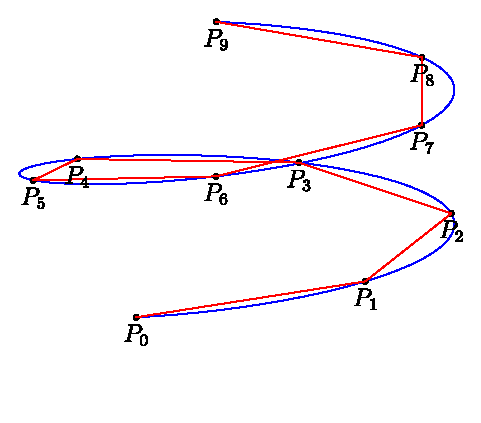
\includegraphics{./cap_curvas/figs/helice_retificacao}
\caption{Aproximação poligonal do comprimento do arco}\label{fig_compr_arc}
\end{figure}

 
 
Seja $a=t_0<t_1<t_2<\cdots<t_n=b $ uma partição equidistante do domínio com $\Delta t=t_i-t_{i-1}$ e $P_i=\vec{r}(t_i)$, $i=0,1,\cdots,n$, pontos sobre a curva, como mostra a figura \ref{fig_compr_arc}. Uma possível aproximação para o comprimento da curva é dado pelo comprimento da poligonal. Observe que o comprimento do segmento $P_{i-1}P_i$ é dado por $\|P_i-P_{i-1}\|$, logo, a aproximação para o comprimento da curva é
\begin{eqnarray*}
L_n&=&\sum_{i=1}^n\|P_i-P_{i-1}\|\\
&=&\sum_{i=1}^n \sqrt{(x_i-x_{i-1})^2+(y_i-y_{i-1})^2+(z_i-z_{i-1})^2}\\
&=&\sum_{i=1}^n \Delta t \sqrt{\frac{(x_i-x_{i-1})^2}{(\Delta t) ^2}+\frac{(y_i-y_{i-1})^2}{(\Delta t) ^2}+\frac{(z_i-z_{i-1})^2}{(\Delta t) ^2}}\\
&=&\sum_{i=1}^n \sqrt{\left(\frac{x_i-x_{i-1}}{\Delta t }\right)^2+\left(\frac{y_i-y_{i-1}}{\Delta t}\right)^2+\left(\frac{z_i-z_{i-1}}{\Delta t}\right)^2}\Delta t.
\end{eqnarray*}
Naturalmente, $L=\lim_{n\to\infty }L_n$. Como o lado direito da última igualdade é uma soma de Riemann, temos:
\begin{equation}\label{defcomparco}
L=\int_{a}^{b} \sqrt{\left(\frac{dx(t)}{dt}\right)^2+\left(\frac{dy(t)}{dt}\right)^2+\left(\frac{dz(t)}{dt}\right)^2}dt=\int_{a}^{b}\|\vec{r}\!~'(t)\|dt.
\end{equation}
Logo, o comprimero do arco $s$ quando a parâmetro corre de $a$ até $t$ é
\begin{equation}\label{defcomparco_1}
s(t)=\int_{a}^{t}\|\vec{r}\!~'(\tau)\|d\tau,\qquad a\leq t\leq b.
\end{equation}

\subsection*{Exercícios resolvidos}

\construirExeresol


\subsection*{Exercícios}

\construirExer



\section{Triedro de Frenet-Serret}

Seja a curva descrita pela função vetorial $\vec{r}(t)$. Queremos encontrar um vetor que seja tangente à curva em um dado ponto\index{vetor tangente}. Para tal tomamos o limite
$$\lim_{h\to 0} \frac{\vec{r}(t+h)-\vec{r}(t)}{h}$$  
Este limite converge para $\vec{r}'(t)$ e, geometricamente, para o vetor tangente à curva no ponto $P$ relativo a $\vec{r}(t)$\footnote{O leitor atento ao formalismo pode tomar esta coma uma definição de vetor tangente. Adiante, veremos que esta definição é consistente com o vetor tangente do cálculo de funções de uma variável.} sempre que $\vec{r}'(t)\neq \vec{0}$. O sentido do vetor $\vec{r}~\!'(t)$ é dado pela parametrização da curva, em outras palavras, o vetor $\vec{r}~\!'(t)$ aponta no sentido em que o parâmetro $t$ cresce.


\begin{figure}%{0.35\textwidth}
\begin{center}
    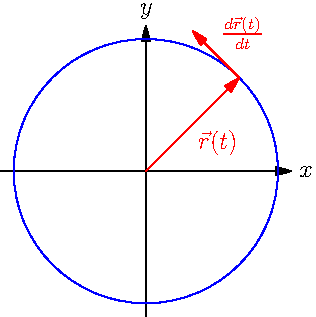
\includegraphics{./cap_curvas/figs/vetor_tangente_circunferencia}
\caption{O vetor tangente $\vec{r}\!~'(t)$}\label{circtang}
  \end{center}
\end{figure}


Observe que a norma do vetor tangente depende de como a curva é parametrizada e não apenas da curva em si. A fim de trabalhar com um objeto que independe da parametrização, é natural definirmos o vetor tangente unitário\index{vetor tangente unitário}, denotado por $\vec{T}$ (veja figura \ref{Frenet_Serret}):
\begin{equation}\label{defvecunit}
\|\vec{T}(t)\|=\frac{\vec{r}\!~'(t)}{\left\|\vec{r}\!~'(t)\right\|},\qquad \vec{r}\!~'(t)\neq \vec{0}.
\end{equation} 
A condição de existência para o vetor $\vec{T}$ é a função vetorial que parametriza a curva seja diferenciável que sua derivada seja diferente de zero, ou seja, que a parametrização seja regular.

\begin{obs} Quando $\vec{r}(t)$ representa a trajetória de uma partícula ao longo do tempo, a derivada $\vec{r}\!~(t)$ é a velocidade $\vec{v}(t)$ da partícula. Neste caso, o vetor tangente unitário é o versor associado a $\vec{v}(t)$:
$$\vec{v}(t)=v(t) \hat{v}(t)=v(t) \vec{T}(t).$$
A norma de $\vec{v}(t)$, denotada por $v(t)$, é chamada de velocidade escalar\index{velocidade escalar}. O vetor $\vec{T}(t)$ indica o sentido e a direção da velocidade.
\end{obs}

O vetor $\vec{T}$ pode ser definido de forma alternativa como segue: olhamos $s$ como função de $t$ na expressão (\ref{defcomparco_1}) e observamos que $s'(t)=\|\vec{r}\!~'(t)\|>0$. Assim, $s(t)$ é uma função contínua e monótona de $t$. Também, usando a rega da cadeia, temos:
$$
\frac{d\vec{r}}{dt}=\frac{d\vec{r}}{ds}\frac{ds}{dt}=\frac{d\vec{r}}{ds}\|\vec{r}\!~'(t)\|.
$$
Como $\vec{r}'(t)$ representa o vetor tangente, então
$$
\frac{d\vec{r}}{ds}=\frac{1}{\|\vec{r}\!~'(t)\|}\frac{d\vec{r}}{dt}=\vec{T}
$$
representa um vetor tangente unitário.


\begin{figure}%{0.35\textwidth}
\begin{center}
    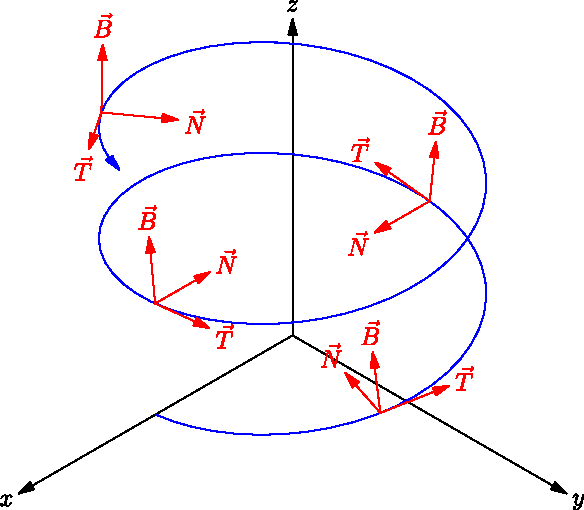
\includegraphics{./cap_curvas/figs/helice_TNB}
\caption{Triedro de Frenet-Serret}\label{Frenet_Serret}
  \end{center}
\end{figure}


Agora, queremos definir um vetor ortogonal a $\vec{T}$ que esteja no mesmo plano formado por $\vec{r}'(t)$ e $\vec{r}''(t)$. Para isso, usamos o resultado do teorema \ref{teodernormacst}. Observe que a função vetorial $\vec{T}(t)$ possui módulo constante e, portanto, $\vec{T}(t)\cdot \vec{T}'(t)=0$. Observe que $\vec{T}(t)$ e $\vec{T}'(t)$ estão ambos no plano formado por $\vec{r}'(t)$ e $\vec{r}''(t)$ e são ortogonais entre si. No entanto, $\vec{T}'(t)$ não é necessariamente unitário. Logo, faz sentido definir o vetor normal unitário\index{vetor normal unitário} como
$$
\vec{N}=\frac{\vec{T}'(t)}{\|\vec{T}'(t)\|}.
$$
A figura \ref{Frenet_Serret} contém a representação do triedro de Frenet-Serret em alguns pontos de uma hélice dextrogira.

Finalmente, vamos definir um vetor unitário que é simultanemente ortogonal a $\vec{T}$ e $\vec{N}$. A forma natural de obter um vetor ortogonal a outros dois vem do produto vetorial. Assim, o vetor binormal unitário\index{vetor binormal unitário} é definido como
$$
\vec{B}=\vec{T}\times\vec{N}.
$$
Das propriedades de produto vetorial, temos que $\vec{B}$, além de ortogonal a $\vec{T}$ e $\vec{N}$, é unitário e forma um sistema dextrogiro. O trio $\vec{T}$, $\vec{N}$ e $\vec{B}$ é chamado de triedro de Frenet-Serret. A figura \ref{Frenet_Serret} apresenta a representação de alguns triedros de Frenet-Serret.


\subsection*{Exercícios resolvidos}

\construirExeresol


\subsection*{Exercícios}

\begin{exer} Represente graficamente o terno de vetores $\vec{T}$,$\vec{N}$ e $\vec{B}$ e verifique através da regra da mão direita as seguintes identidades:
\begin{itemize}
\item[a)]$\vec{B}=\vec{T}\times\vec{N}$
\item[b)]$\vec{T}=\vec{N}\times\vec{B}$
\item[c)]$\vec{N}=\vec{B}\times\vec{T}$
\end{itemize}
Use a identidade vetorial dada por
$$\vec{u}\times\left(\vec{v}\times\vec{w}\right)=\vec{v}\left(\vec{u}\cdot\vec{w}\right)-\vec{w}\left(\vec{u}\cdot\vec{v}\right)$$ para obter as identidades $b$ e $c$ a partir de $a$.
\end{exer}


\begin{exer} Considere a trajetória dada pela equações paramétricas
\begin{eqnarray*}
x&=&t\sin (t)\\
y&=&t\cos (t)\\
z&=&0
\end{eqnarray*}
Esboce gráfico dessa trajetória para $0\leq t \leq 2\pi$, indicando os pontos inicial e final. Esboce o triedro $\vec{T}$, $\vec{N}$ e $\vec{B}$ no instante $t=\pi/2$.(Obs.: Não é necessário calcular analiticamente o triedro.) Considere a identidade vetorial $\frac{d r^2}{dt}=2\vec{r}\cdot\frac{d\vec{r}}{dt}$ no instante $t=\pi/2$, ela é compatível com seu desenho?
\end{exer}

\begin{exer} Um erro comum entre estudantes é substituir a definição de vetor binormal unitário $\vec{B}=\vec{T}\times\vec{N}$ pela expressão espúria dada por $$\frac{\frac{d\vec{N}}{dt}}{\left\|\frac{d\vec{N}}{dt}\right\|}.$$ Calcule esta expressão para o movimento circular uniforme e verifique que ela é igual a $-\vec{T}$ e, portanto, perpendicular a $\vec{B}$.
\end{exer}


\construirExer


\section{Curvatura e Torção}

Nessa seção, estamos interessados em definir, a cada ponto da curva, funções que medem o quanto ela está torcida ou curvada, isto é, se a curva é muito diferente de uma reta ou se está fora de qualquer plano do espaço. Primeiro, definiremos uma função chamada de curvatura\index{curvatura}, que mede a cada ponto do domínio, a variação do vetor tangente com respeito ao comprimento de arco $s$. Naturalmente, queremos que a reta tenha curvatura nula, pois ela não difere da sua tangente em ponto algum. Para facilitar a visualização, podemos começar pensando apenas nas curvas que estão contidas em algum plano. A figura \ref{curvatura} nos dá uma ideia de curvatura.


\begin{figure}
\begin{center}
    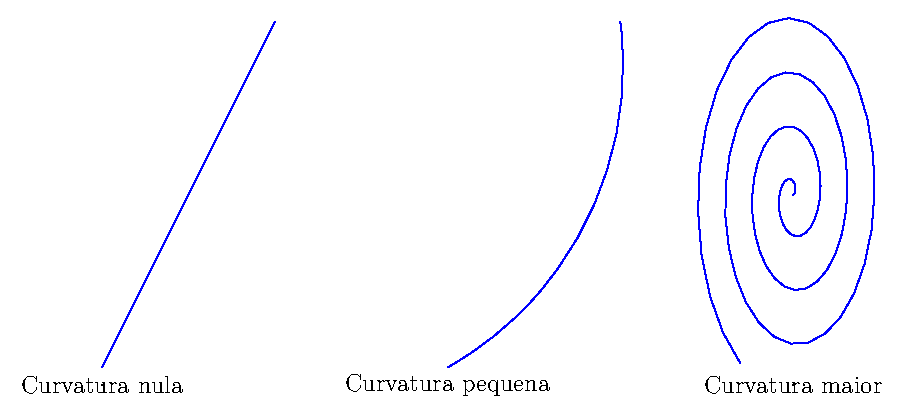
\includegraphics{./cap_curvas/figs/exemplos_de_curvatura}
 \caption{Ideia de curvatura.\label{curvatura}}
  \end{center}
\end{figure}
 
Pelo teorema \ref{teodernormacst}, temos que $\frac{d \vec{T} }{ds}$ é paralelo ao vetor normal $\vec{N}$, ou seja,
\begin{equation}{\label{Frenet_1}}
\frac{d \vec{T} }{ds}=\kappa   \vec{N},
\end{equation}
onde $\kappa(t)>0$ é uma função escalar chamada de curvatura. Por outro lado, calculamos a variação do vetor tangente com respeito ao comprimento de arco $s$ usando a regra da cadeia
$$
\frac{d \vec{T} }{ds}=\frac{d \vec{T} }{dt}\frac{dt}{ds}=\frac{d \vec{T} }{dt}\frac{1}{|s'(t)|},
$$
onde $s(t)$ é a função que mede o comprimento do arco dado pela expressão (\ref{defcomparco_1}). Usando o fato que $s'(t)=\|\vec{r}'(t)\|$, temos:
$$
\frac{d \vec{T} }{ds}=\frac{1}{\|\vec{r}'(t)\|}\frac{d \vec{T} }{dt}.
$$
Portanto, podemos escrever
$$
\kappa(t)=\frac{\|\vec{T}'(t)\|}{\|\vec{r}'(t)\|}.
$$

Definimos também, para cada ponto $t$ do domínio, o raio de curvatura\index{raio de curvatura} $\rho(t)$ da forma:
$$
\rho(t)=\frac{1}{\kappa(t)}.
$$
O raio de curvatura tem a seguinte interpretação geométrica: considere um ponto $\vec{r}(t_0)$ onde da curvatura não é nula e defina o ponto $\vec{r}(t_0)+\kappa(t_0)\vec{N}$, chamado de centro de curvatura\index{centro de curvatura}. O círculo centrado no centro de curvatura e raio $\rho(t_0)$ é tangente a curva em $t_0$ e possui a mesma curvatura (veja a figura \ref{raio_de_curvatura}).


\begin{figure}
\begin{center}
    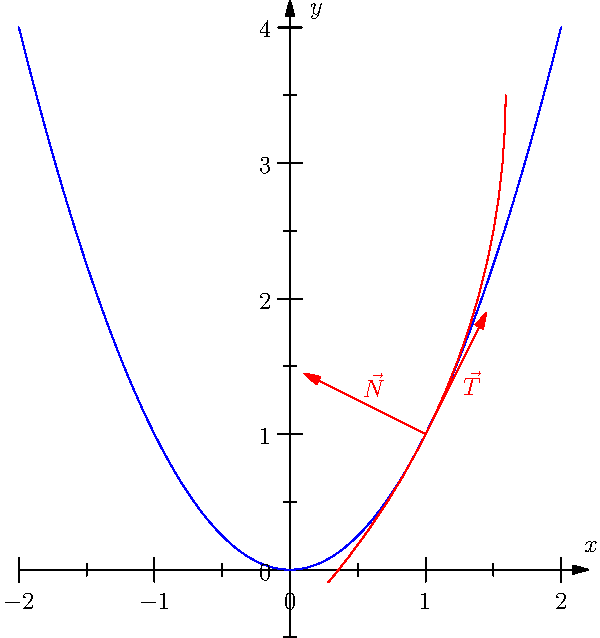
\includegraphics{./cap_curvas/figs/circulo_curvatura_parabola}
 \caption{Círculo de curvatura}\label{raio_de_curvatura}
  \end{center}
\end{figure}

\begin{ex}A curva descrita por $\vec{r}=a\cos(t)\vec{i}+a\sin(t)\vec{j},\qquad a>0,\ 0\leq t\leq 2\pi$ é uma cincunferência. Sua curvatura pode ser obtida da seguinte forma:
\begin{eqnarray}
 \vec{r}'(t)&=&-a\sin(t)\vec{i}+a\cos(t)\vec{j},\\
 \|\vec{r}'(t)\|&=&\sqrt{a^2\sin^2(t)+a^2\cos^2(t)}=\sqrt{a^2}=|a|=a,\\
 \vec{T}(t)&=&\frac{-a\sin(t)\vec{i}+a\cos(t)\vec{j}}{a}=-\sin(t)\vec{i}+\cos(t)\vec{j},\\
\end{eqnarray}

\end{ex}
\begin{ex}Dada a curva $y=x^2$, vamos encontrar a curvatura e o raio de curvatura no ponto $x=1$. Primeiro, encontramos uma parametrização para essa curva, por exemplo, $\vec{r}=t\vec{i}+t^2\vec{j}$. Calculamos:
$$
\vec{r}'(t)=\vec{i}+2t\vec{j},
$$
$$
\|\vec{r}'(t)\|=\sqrt{1+4t^2},
$$
$$
\vec{T}(t)=\frac{1}{\sqrt{1+4t^2}}\left(\vec{i}+2t\vec{j}\right)
$$
e
$$
\vec{T}'(t)=-\frac{4t}{\sqrt{(1+4t^2})^3}\vec{i}+\left(-\frac{8t^2}{\sqrt{(1+4t^2})^3}+\frac{2}{\sqrt{1+4t^2}}\right)\vec{j},
$$
Em $t=1$, temos:
$$
\|\vec{r}'(t)\|=\sqrt{5},
$$
$$
\vec{T}'(t)=-\frac{4}{\sqrt{5^3}}\vec{i}+\left(-\frac{8}{\sqrt{5^3}}+\frac{2}{\sqrt{5}}\right)\vec{j}=-\frac{4}{\sqrt{5^3}}\vec{i}+\frac{2}{\sqrt{5^3}}\vec{j},
$$
e
$$
\|\vec{T}'(t)\|=\sqrt{\frac{16}{5^3}+\frac{4}{5^3}}=\frac{2}{5}.
$$
Portanto,
$$
\kappa(1)=\frac{\|\vec{T}'\|}{\|\vec{r}'\|}=\frac{2}{5\sqrt{5}}
$$
e
$$
\rho(1)=\frac{5\sqrt{5}}{2}.
$$
veja representação geométrica na figura \ref{raio_de_curvatura}.
\end{ex}

O leitor deve ter observado que conhecendo somente a curvatura não é possível reconstruir uma curva a partir de um ponto dado. Um curva pode não estar contida em plano algum no espaço e, por isso, precisamos definir uma função escalar, chamada torção, que mede a magnitude da variação do vetor binormal. A figura \ref{torcao} apresenta uma ideia de torção\index{torção}: uma curva contida em algum plano no espaço tem torção nula e quando maior a variação com respeito ao plano definido por $\vec{T}$ e $\vec{N}$, maior a torção. O leitor deve tomar cuidado na interpretação da figura \ref{torcao}, pois se esticarmos indefinidamente a hélice circular representada, ela voltará a se aproximar de uma reta, que tem torção nula (veja problema \ref{prob_torcao}). Sabendo que a torção será definida em termos da variação do vetor binormal com respeito ao comprimento de arco $s(t)$, fazendo algumas observações:
$$
\frac{d\vec{B}}{ds}=\frac{d}{ds}\left(\vec{T}\times\vec{N}\right)=\frac{d\vec{T}}{ds}\times \vec{N}+\vec{T}\times\frac{d\vec{N}}{ds}.
$$
Usando a expressão (\ref{Frenet_1}), temos que $\frac{d\vec{T}}{ds}=\kappa\vec{N}$, logo 
$$
\frac{d\vec{B}}{ds}=\vec{T}\times\frac{d\vec{N}}{ds}.
$$
Isso implica que $\frac{d\vec{B}}{ds}$ é ortogonal a $\vec{T}$. Mas, pelo teorema \ref{teodernormacst}, temos que $\frac{d\vec{B}}{ds}$ é ortogonal a $\vec{B}$. Logo, $\frac{d\vec{B}}{ds}$ é paralelo a $\vec{N}$, ou seja,
\begin{equation}{\label{Frenet_2}}
\frac{d\vec{B}}{ds}=-\tau\vec{N},
\end{equation}
onde $\tau$ é chamado de torção\index{torção}. O sinal negativo tem um propósito: quando $\tau>0$, $\frac{d\vec{B}}{ds}$ está no sentido de $-\vec{N}$; então se $P$ é um ponto sobre a curva movendo-se no sentido positivo, $\vec{B}$ gira em torno de $\vec{T}$ como um parafuso de rosca direita sendo apertado (veja a figura \ref{Curvatura_torcao_1}). Em alguns contextos, calculamos a módulo da torção, dada por
$$
|\tau|=\left\|\frac{d\vec{B}}{ds}\right\|=\frac{\|\vec{B}'(t)\|}{\|\vec{r}'(t)\|}.
$$


\begin{figure}
\begin{center}
    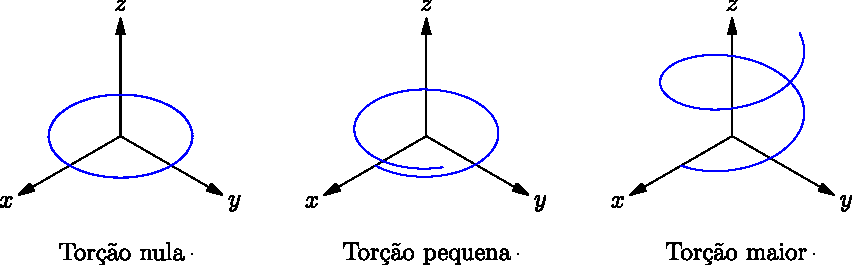
\includegraphics{./cap_curvas/figs/exemplos_de_torcao}
 \caption{Ideia de torção.}\label{torcao}
  \end{center}
\end{figure}



Ainda, definimos o raio de torção\index{raio de torção} por
$$
\sigma(t)=\frac{1}{\tau(t)}.
$$

Podemos calcular $\frac{d\vec{N}}{ds}$ em termos da curvatura e da torção:
\begin{equation*}
\frac{d\vec{N}}{ds}=\frac{d}{ds}\left(\vec{B}\times\vec{T}\right)=\frac{d\vec{B}}{ds}\times \vec{T}+\vec{B}\times\frac{d\vec{T}}{ds}.
\end{equation*}
Usando as expressões (\ref{Frenet_1}) e (\ref{Frenet_2}), escrevemos
\begin{equation*}
\frac{d\vec{N}}{ds}=-\tau\vec{N} \times \vec{T}+\vec{B}\times \kappa \vec{N}.
\end{equation*}
ou seja,
\begin{equation}{\label{Frenet_3}}
\frac{d\vec{N}}{ds}=-\kappa \vec{T}+\tau \vec{B}.
\end{equation}
As equações (\ref{Frenet_1}), (\ref{Frenet_2}) e (\ref{Frenet_3}) são chamadas de Fórmulas de Frenet-Serret.

Como esperávamos, se $\kappa=0$, então $\frac{d\vec{T}}{ds}=\vec{0}$, o que implica que $\vec{T}$ não varia ao longo da curva, ou seja, a curva é uma reta. Agora, se $\tau=0$, então $\frac{d\vec{B}}{ds}=\vec{0}$ e $\vec{B}$ é um vetor constante. Como $\vec{B}\cdot \vec{T}=\vec{B}\cdot \frac{d\vec{r}}{ds}=0$, então podemos integrar para obter $\vec{B}\cdot (\vec{r}-\vec{r_0})=0$, onde $r_0$ é um vetor constante da integração. Logo $\vec{r}$ está contido no plano ortogonal a $\vec{B}$.



\begin{ex} Vamos calcular curvatura, raio de curvatura e o módulo da torção para a hélice circular $\vec{r}(t)=\cos(t)\vec{i}+\sin(t)+t\vec{k}$:
$$
\vec{r}'(t)=-\sin(t)\vec{i}+\cos(t)+\vec{k},
$$
$$
\|\vec{r}'(t)\|=\sqrt{2},
$$
$$
\vec{T}(t)=-\frac{\sin(t)}{\sqrt{2}}\vec{i}+\frac{\cos(t)}{\sqrt{2}}+\frac{1}{\sqrt{2}}\vec{k},
$$
$$
\vec{T}'(t)=-\frac{\cos(t)}{\sqrt{2}}\vec{i}-\frac{\sin(t)}{\sqrt{2}},
$$
$$
\|\vec{T}'(t)\|=\frac{1}{\sqrt{2}},
$$
$$
\kappa(t)=\frac{1}{\sqrt{2}}\cdot \frac{1}{\sqrt{2}}=\frac{1}{2},
$$
$$
\rho(t)=2,
$$
$$
\vec{N}(t)=-\cos(t)\vec{i}-\sin(t)\vec{j},
$$
\begin{eqnarray*}
\vec{B}(t)&=&\left|\begin{array}{ccc}\vec{i}&\vec{j}&\vec{k}\\-\frac{\sin(t)}{\sqrt{2}}&\frac{\cos(t)}{\sqrt{2}}&\frac{1}{\sqrt{2}}\\-\cos(t)&-\sin(t)&0\end{array}\right|\\
&=&\frac{\sin(t)}{\sqrt{2}}\vec{i}-\frac{\cos(t)}{\sqrt{2}}\vec{j}+\frac{1}{\sqrt{2}}\vec{k}.
\end{eqnarray*}
$$
\vec{B}'(t)=\frac{\cos(t)}{\sqrt{2}}\vec{i}+\frac{\sin(t)}{\sqrt{2}}\vec{j},
$$
$$
\|\vec{B}'(t)\|=\frac{1}{\sqrt{2}},
$$
$$
|\tau(t)|=\frac{1}{2}.
$$
\end{ex}

\begin{exer} Calcule a curvatura, o raio de curvatura e o módulo da torção das curvas abaixo:
\begin{itemize}
\item[a)] $\vec{r}=a\cosh(t)\vec{i}+b\sinh(t)\vec{j}$, $-\infty<t<\infty$, $a>0,\ b>0$.
\item[b)] $\vec{r}=a\cos(t)\vec{i}+b\sin(t)\vec{k}$, $0\leq t\leq 2\pi$, $a>0,\ b>0$.
\item[c)] $\vec{r}=a\cos(t)\vec{i}+a\sin(t)+ct\vec{k}$, $t\geq 0$, $a>0,\ c>0$.

\end{itemize}
\end{exer}
 
 \begin{exer}{\label{prob_torcao}} Dada a hélice circular $\vec{r}=a\cos(t)\vec{i}+a\sin(t)+ct\vec{k}$, $t\geq 0$, $a>0,\ c>0$, calcule o valor de $c$ para que a torção seja máxima.
 \end{exer}


 
 \begin{figure}
\begin{center}
    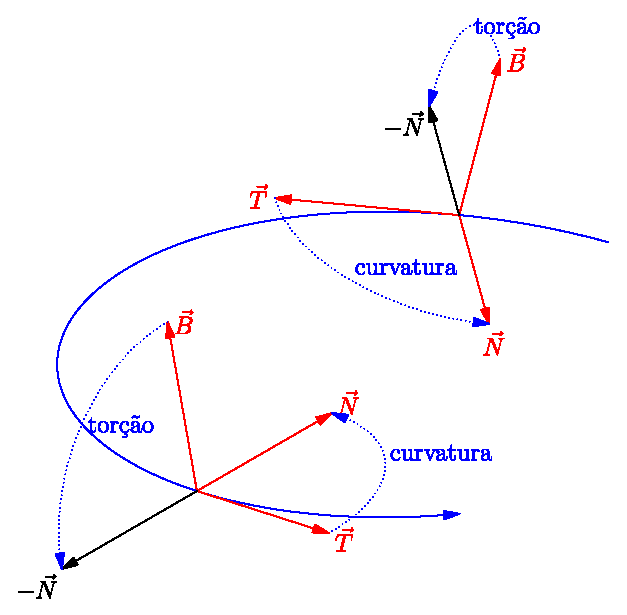
\includegraphics{./cap_curvas/figs/curvatura_torcao}
 \caption{Curvatura e Torção}\label{Curvatura_torcao_1}
  \end{center}
\end{figure}


A curvatura e a torção podem ser calculadas de maneira mais simples. Para concluir isso, começamos calculando as derivadas de $\vec{r}$. Usamos aqui que $s'(t)=\|\vec{r}'(t)\|$, obtida da equação (\ref{defcomparco_1}):
$$
\vec{r}'=\frac{d\vec{r}}{ds}\frac{ds}{dt}=s' \vec{T},
$$
\begin{eqnarray*}
\vec{r}''&=&s'' \vec{T}+s' \vec{T}'\\&=&s'' \vec{T}+s' \|\vec{T}'\|\vec{N}\\
&=&s'' \vec{T}+s'^2 \kappa \vec{N}
\end{eqnarray*}
e
\begin{eqnarray*}
\vec{r}'''&=&s''' \vec{T}+s''\vec{T}'+2s's''\kappa \vec{N}+s'^2 \left(\kappa \vec{N}'+\kappa' \vec{N}\right)\\
&=&s''' \vec{T}+s''s'\kappa \vec{N}+\left(2s's''\kappa+s'^2\kappa'\right) \vec{N}\\
&+&s'^3 \kappa (-\kappa \vec{T}+\tau\vec{B})\\
&=&\left(s'''-\kappa^2s'^3\right) \vec{T}+\left(3s''s'\kappa +s'^2\kappa'\right)\vec{N}+s'^3 \kappa \tau\vec{B},
\end{eqnarray*}
onde usamos as expressões (\ref{Frenet_1}) e (\ref{Frenet_3}). Agora, tomamos os seguintes produtos:
$$
\vec{r}'\times \vec{r}''=s'^3\kappa \vec{B}\qquad\text{e}\qquad
\vec{r}'\times \vec{r}''\cdot \vec{r}'''=s'^6\kappa^2\tau.
$$
Isso implica em 
$$
\|\vec{r}'\times \vec{r}''\|=|s'|^3\kappa\qquad\text{e}\qquad
\vec{r}'\times \vec{r}''\cdot \vec{r}'''=\|\vec{r}'\times \vec{r}''\|^2\tau.
$$
ou seja,
\begin{equation}{\label{curvatura_2}}
\kappa =\frac{\|\vec{r}'\times \vec{r}''\|}{\|r'\|^3}
\end{equation}
e
\begin{equation}{\label{torcao_2}}
\tau=\frac{\vec{r}'\times \vec{r}''\cdot \vec{r}'''}{\|\vec{r}'\times \vec{r}''\|^2}.
\end{equation}

\begin{obs}\index{aceleração!normal}\index{aceleração!tangencial}Uma aplicação natural é a decomposição da aceleração em suas componentes tangencial e normal. Observe que
$$
\vec{r}'=\vec{v}=v\vec{T}=s' \vec{T}
$$
e
$$
\vec{a}=v' \vec{T}+v^2 \kappa \vec{N}.
$$
Concluímos que a aceleração está no plano normal a $\vec{B}$ e possui componentes tangencial e normal:
$$
\vec{a}=a_T \vec{T}+a_N \vec{N},
$$
onde $a_T=v'$ e $a_N=v^2\kappa$. Então, se a velocidade possui normal constante, temos que $v'=0$ e a aceleração possui apenas componente normal.

\end{obs}


\begin{ex} Consideremos agora, a curva gerada pelas seguintes equações paramétricas:
$$x(t)=\cos(t)\qquad y(t)=\sin(t)\qquad z(t)=f(t).$$
 Onde $f(t)$ é uma função dada. Observe que a projeção desta curva no plano $xy$ é uma circuferência de raio 1. A curva é, portanto, gerada pela trajetória de ponto cuja projeção do movimento no plano $xy$ é cirvular e a altura é dada pela função $f(t)$. Podemos calcular a curvatura e a torção conforme a seguir:
 \begin{eqnarray*}
  \vec{r}(t)&=&\cos(t)\vec{i}+\sin(t)\vec{j}+f(t)\vec{k}\\
  \vec{r'}(t)&=&-\sin(t)\vec{i}+\cos(t)\vec{j}+f'(t)\vec{k}\\
  \vec{r''}(t)&=&-\cos(t)\vec{i}-\sin(t)\vec{j}+f''(t)\vec{k}\\
  \vec{r'''}(t)&=&\sin(t)\vec{i}-\cos(t)\vec{j}+f'''(t)\vec{k}
 \end{eqnarray*}
Assim, calculamos:
 \begin{eqnarray*}
  \vec{r'}(t)\times\vec{r''}(t) &=&\left[f''(t)\cos(t)+f'(t)\sin(t)\right]\vec{i}+\left[-f'(t)\cos(t)+f''(t)\sin(t)\right]\vec{j}+\vec{k}\\
 \vec{r'}(t)\times\vec{r''}(t)\cdot r'''(t)&=&f'(t)+f'''(t)\\
 \|\vec{r'}(t)\times\vec{r''}(t)\|&=&\sqrt{1+\left(f'(t)\right)^2+\left(f''(t)\right)^2}\\
 \|\vec{r'}(t)\|&=&\sqrt{1+\left(f'(t)\right)^2}
 \end{eqnarray*}
E finalmente, obtemos:
 \begin{eqnarray*}
\kappa&=&\frac{\sqrt{1+\left(f'(t)\right)^2+\left(f''(t)\right)^2}}{\left({1+\left(f'(t)\right)^2}\right)^{3/2}}\\
\tau&=&\frac{f'(t)+f'''(t)}{1+\left(f'(t)\right)^2+\left(f''(t)\right)^2}
 \end{eqnarray*}
Podemos, agora, explorar diversos casos particular:
\begin{itemize}
 \item [a)] Caso $f(t)=c$ constante. Neste caso, recaímos na circunferência de raio 1, cuja curvatura é 1 e a torção é nula.
 \item [b)] Caso $f(t)=ct$ com $c$ constante. Recaímos na hélice cicular uniforme, já estudada, cuja curvatura é $\frac{1}{1+c^2}$ e a torção é $\frac{c}{1+c^2}$.
 \item [c)] Caso $f(t)=ct^2$ com $c$ constante. Recaímos na hélice cicular com espaçamento linearmente crescente, cuja curvatura é dada por ${\frac {\sqrt {4\,{c}^{2}+1+4\,{c}^{2}{t}^{2}}}{ \left( 1+4\,{c}^{2}{t
}^{2} \right) ^{3/2}}}$ e cuja torção é dada por $2\,{\frac {ct}{4\,{c}^{2}+1+4\,{c}^{2}{t}^{2}}}$.
 \item [d)] Caso $f(t)=\sin(t)$. Recaímos na elipse de semieixos $1$ e $\sqrt{2}$ no plano $y=z$. Neste caso, a curvatura é $\kappa=\frac{\sqrt{2}}{\left(1+\cos(t)^2\right)^{3/2}}$ e a torção é nula.
 \item [e)] Caso $\tau=0$, isto é, $f'(t)+f'''(t)=0$, o que é equivalente a $f(t)=a+b\cos(t)+c\sin(t)$ onde $a$, $b$ e $c$ são constantes. Recaímos na elipse de semieixos $1$ e $\sqrt{1+b^2+c^2}$ no plano $z=bx+cy$. Neste caso, a curvatura é $\kappa={\frac {\sqrt {b^2+c^2+1}}{\left(1-bc\sin(2t)+c^2\cos^2(t)+b^2\sin^2(t) \right) ^{3/2}}}$ e a torção é nula.
  \end{itemize}
\end{ex}


\subsection*{Exercícios resolvidos}

\construirExeresol


\subsection*{Exercícios}
\begin{exer}
Considere as funções vetoriais dadas por
\begin{eqnarray*}
\vec{f}(t)&=&\cos(\pi t)\vec{i}+\sin(\pi t)\vec{j}\\
\vec{g}(t)&=&\cos(\pi t^3)\vec{i}+\sin(\pi t^3)\vec{j}
\end{eqnarray*}
Verifique que ambas parametrizam a mesma curva quando $-1\leq t \leq 1$. Verifique se as parametrizações são regulares e compare o comportamento da derivada em $t=0$. Que consequências isso tem para a existência do vetor tangente unitário? 
\end{exer}


\begin{exer}Calcule curvatura e torção para a curva $\vec{r}=a\cos(t)\vec{i}+a\sin(t)\vec{j}+ct\vec{k}$, $a>0$, $c>0$, $t>0$ usando as expressões (\ref{curvatura_2}) e (\ref{torcao_2}).
\end{exer}

\begin{exer}Uma motocicleta percorre uma trajetória circular de raio $20m$ com velocidade constante em módulo. A motocicleta poderá derrapar se a aceleração normal exceder $2m/s^2$. Qual é a velocidade máxima do motocicleta para que ela não derrape?
\end{exer}

  
  
\begin{exer} Mostre que se $a_N$ e $a_T$ indicam as acelerações normal e tangencial, respectivamente, então
$$\|\vec{a}\|^2=a_N^2+a_T^2$$
onde $\vec{a}$ é o vetor aceleração.
\end{exer}
\begin{resp}
 \begin{eqnarray}
\|\vec{a}\|^2&=&\vec{a}\cdot\vec{a}=\left(a_T\vec{T}+a_N\vec{N}\right)\cdot\left(a_T\vec{T}+a_N\vec{N}\right)\\
&=&a_T^2\vec{T}\cdot\vec{T}+a_Na_T\vec{T}\cdot\vec{N}+a_Ta_N\vec{T}\cdot\vec{N}+A_N^2\vec{T}\cdot\vec{T}  
 \end{eqnarray}

\end{resp}


\construirExer




% 
%\end{document}